\documentclass[12pt,twoside,a4paper]{book}


\usepackage[utf8]{inputenc}
\usepackage[T1]{fontenc}
\usepackage{lmodern}
\usepackage{amsmath,amssymb,amsthm}
\usepackage{mathabx}\changenotsign
\usepackage{mathrsfs}
\usepackage{dsfont}
\usepackage[babel]{microtype}
\usepackage{xcolor}  	
\usepackage[backref]{hyperref}
\usepackage{mathtools}
\usepackage{indentfirst}
\usepackage{graphicx} % Gerencia imagens incluidas

\hypersetup{
	colorlinks,
    linkcolor={red!60!black},
    citecolor={green!60!black},
    urlcolor={blue!60!black},
}

\usepackage{bookmark}

\usepackage[abbrev,msc-links,backrefs]{amsrefs}
\usepackage{doi}
\renewcommand{\doitext}{DOI\,}

\renewcommand{\PrintDOI}[1]{\doi{#1}}

\renewcommand{\eprint}[1]{\href{http://arxiv.org/abs/#1}{arXiv:#1}}


\usepackage[T1]{fontenc}
\usepackage{lmodern}

\usepackage[english]{babel}
\numberwithin{equation}{section}

\linespread{1.3}
\usepackage{amsfonts}
\usepackage{geometry}
\geometry{left=27.5mm,right=27.5mm, top=25mm, bottom=25mm}


\usepackage{enumitem}
\def\rmlabel{\upshape({\itshape \roman*\,})}
\def\RMlabel{\upshape(\Roman*)}
\def\alabel{\upshape({\itshape \alph*\,})}
\def\Alabel{\upshape({\itshape \Alph*\,})}
\def\nlabel{\upshape({\itshape \arabic*\,})}

\def\aplabel{\upshape({\itshape \alph*\,$'$})}

\let\polishlcross=\l
\def\l{\ifmmode\ell\else\polishlcross\fi}

\def\tand{\ \text{and}\ }
\def\qand{\quad\text{and}\quad}
\def\qqand{\qquad\text{and}\qquad}

\let\emptyset=\varnothing
\let\setminus=\smallsetminus
\let\backslash=\smallsetminus
\let\subset\subseteq
\let\log=\ln

\newcommand\mc{\mathop{\textrm{\rm mc}}\nolimits}

\makeatletter
\def\moverlay{\mathpalette\mov@rlay}
\def\mov@rlay#1#2{\leavevmode\vtop{   \baselineskip\z@skip \lineskiplimit-\maxdimen
   \ialign{\hfil$\m@th#1##$\hfil\cr#2\crcr}}}
\newcommand{\charfusion}[3][\mathord]{
    #1{\ifx#1\mathop\vphantom{#2}\fi
        \mathpalette\mov@rlay{#2\cr#3}
      }
    \ifx#1\mathop\expandafter\displaylimits\fi}
\makeatother

\DeclareMathOperator{\dom}{{\rm dom}}

\newcommand{\dcup}{\charfusion[\mathbin]{\cup}{\cdot}}
\newcommand{\bigdcup}{\charfusion[\mathop]{\bigcup}{\cdot}}


\DeclareFontFamily{U}  {MnSymbolC}{}
\DeclareSymbolFont{MnSyC}         {U}  {MnSymbolC}{m}{n}
\DeclareFontShape{U}{MnSymbolC}{m}{n}{
    <-6>  MnSymbolC5
   <6-7>  MnSymbolC6
   <7-8>  MnSymbolC7
   <8-9>  MnSymbolC8
   <9-10> MnSymbolC9
  <10-12> MnSymbolC10
  <12->   MnSymbolC12}{}
\DeclareMathSymbol{\powerset}{\mathord}{MnSyC}{180}



\makeatletter
\def\namedlabel#1#2{\begingroup
    #2%
    \def\@currentlabel{#2}%
    \phantomsection\label{#1}\endgroup
}
\makeatother


\newtheorem{theorem}             {Theorem}[section]
\newtheorem{lemma}     	[theorem] {Lemma}
\newtheorem{conjecture}	[theorem] {Conjecture}
\newtheorem{property}  	[theorem] {Property}
\newtheorem{definition}	[theorem] {Definition}
\newtheorem{proposition}[theorem] {Proposition}
\newtheorem{corollary}	[theorem] {Corollary}
\newtheorem{fact}	[theorem] {Fact}
\newtheorem{claim}	[theorem] {Claim}

\newtheoremstyle{remark}  {2pt}  {4pt}  {\rm}  {}  {\bfseries}  {.}  {.3em}          {}
\theoremstyle{remark}
\newtheorem{remark}	[theorem] {Remark}
\newtheorem{example}	[theorem] {Example}

\renewcommand{\thefootnote}{\fnsymbol{footnote}}

\let\eps=\varepsilon
\let\theta=\vartheta
\let\rho=\varrho
\let\phi=\varphi


\def\NN{\mathds N}
\def\ZZ{\mathds Z}
\def\QQ{\mathds Q}
\def\RR{\mathds R}
\def\PP{\mathds P}
\def\EE{\mathds E}

\def\cB{\mathcal B}
\def\cR{\mathcal R}

\def\ra{\longrightarrow}
\usepackage{centernot}
\def\nra{\centernot\longrightarrow}
\def\red{\text{\rm red}}
\def\blue{\text{\rm blue}}
\def\green{\text{\rm green}}
\def\R{\text{\rm red}}
\def\B{\text{\rm blue}}

\usepackage{datetime}
\usepackage{lineno}
\newcommand*\patchAmsMathEnvironmentForLineno[1]{%
\expandafter\let\csname old#1\expandafter\endcsname\csname #1\endcsname
\expandafter\let\csname oldend#1\expandafter\endcsname\csname end#1\endcsname
\renewenvironment{#1}%
{\linenomath\csname old#1\endcsname}%
{\csname oldend#1\endcsname\endlinenomath}}%
\newcommand*\patchBothAmsMathEnvironmentsForLineno[1]{%
\patchAmsMathEnvironmentForLineno{#1}%
\patchAmsMathEnvironmentForLineno{#1*}}%
\AtBeginDocument{%
\patchBothAmsMathEnvironmentsForLineno{equation}%
\patchBothAmsMathEnvironmentsForLineno{align}%
\patchBothAmsMathEnvironmentsForLineno{flalign}%
\patchBothAmsMathEnvironmentsForLineno{alignat}%
\patchBothAmsMathEnvironmentsForLineno{gather}%
\patchBothAmsMathEnvironmentsForLineno{multline}%
}
\usepackage{graphicx}
\begin{document}
%\linenumbers

%\title{Extremal and Probabilistic Combinatorics}

\begin{center}
{\bf Extremal and Probabilistic Combinatorics}\\
\vspace{2cm}
Diogo Eduardo Lima Alves\\
\vspace{3cm}

PROJETO DE GRADUAÇÃO EM COMPUTAÇÃO PRESENTED\\
TO\\
CENTRO DE MATEMÁTICA, COMPUTAÇÃO E COGNIÇÃO\\
OF\\
UNIVERSIDADE FEDERAL DO ABC\\
FOR\\
OBTAINING TITLE\\
OF\\
BACHAREL EM CIÊNCIA DA COMPUTAÇÃO\\
\vspace{4cm}
Advisor: Prof. Dr. Guilherme Oliveira Mota\\
\vfill
Santo André, Agosto de 2018
\end{center}

\chapter{Introduction}
Computer Science is truly fundamental for the fast development of Science in the last century, also being fundamental for its validation and communication. It is really hard to think about actual Science without the use of computers or strong science communities connected and accessible by the internet. Computer Science is also essential for the business. All multinational company is also a software company since the way of production, operating and delivering products are managed by software and these aspects are determinants for the success level of any company in the world, it is also not uncommon that one of the most valuable assets of a company can be connected to data, software and algorithms. In this scenario, graphs are also very interesting due its importance to Computer Science.

Graphs are one of the most flexible structures, even for math theory either for efficient algorithms, impacting the study of Algebra, Probability and Combinatorics. They can be used even for modeling many real scenarios in a very easy understandable graphical scheme whose properties can be explored to obtain many useful information what explains its huge importance for many knowledge areas not directly connected to Computer Science or Math Theory.   

This project, more specifically, focus on classical results of Extremal Combinatorics Theory and Graph Theory. It has detailed ideas and explanations about theorems and concepts of a large period of time which have already been intensively studied.

Extremal Combinatorics studies the maximum or minimum size a collection of objects can be at the same time it satisfies certain restrictions. Here these objects will be focus on graphs and graphs' substructures. 

Ramsey Theory is the study of finding order in chaos and, in general, solves mathematical equations in the integers.

Extremal Graph Theory studies graphs' size, as the number interval of edges and vertices, since a specific substructure is forbidden inside the main graph.


%\chapter{Justification}
%ME INTERESSEI PELO TEMA, APENAS!


%\chapter{Objectives}



\chapter{Methodology}
The main bibliography referential material used in this project is the book ``Extremal and Probabilistic Combinatorics'' written by Robert Morris and Roberto Imbuzeiro Oliveira which is part of Impa's mathematical publications and is a result of a Extremal Combinatorics course.

Almost all the doubts and problems about proofs, explanations and structure over the entire text construction was supported by the projects' advisor, the professor Dr. Guilherme Oliveira Mota.



\chapter{Ramsey's Theory}
{\bf Motivational Example:}

``Given a group of 6 people, show that at least 3 people are mutual friends or at least 3 people are mutual strangers''

It is possible to suppose without loss of generality that Richard knows at least three people, Maria, Bete and Jack. If any pair of this friends know each other then it is formed a friendly triangle, otherwise Maria, Bete and Jack form a unfriendly triangle themselves. Replacing people by vertices and a friend relationship by colors (if friends color blue else color red) we realize that with 6 peoples we always have a monochromatic triangle independently the way we construct it, but what about 5 people?

The $K_5$ can be constructed without a monochromatic triangle, this shows that Ramsey number cannot be less than 6, what can be written as  R(3,3) = 6.
\begin{definition}\label{def:RamseyNumbers}
$R(s,t) = n :=$ The minimum $n$ such that any 2-colouring on $K_n$ must have either a complete subgraph $K_s$ whose edges are monochromatic in color 1 or a complete subgraph $K_t$ whose edges are monochromatic in color 2.
\end{definition}

\begin{theorem}\label{thm:RamseyTheorem} 
(Ramsey's Theorem). Let $r \geq 1$. Every colouring $c\colon \dbinom{\mathbb{N}}{2}$ $\rightarrow$ $[r]$ of the pairs in $\mathbb{N}$ contains an infinite monochromatic subset.
\end{theorem}

In order to prove this theorem, it is needed only the pigeonhole principle as it follows:

``If a infinite number of letters lie in a finite number of pigeonholes, then some pigeonhole must contain an infinite number of letters''

Explanation: It is not hard to think about it. Imagine we have a finite number of parts to divide $\mathbb{N}$ whose elements are infinite, let the number of parts be r. We can start giving part 1 a finite quantity of elements, doing the same for parts $\{2, 3,..., r-1\}$. So at this point we have $\{1,2,3,...,r-1\}$ being a set of parts with a finite number of elements, but |$\mathbb{N}$| = $\infty$ and once $|\{1, 2, 3,..., r-1\}|$ is finite we still have infinite elements and only one part to use, so at least one of these parts must have infinite elements.

Given a colouring $c\colon\dbinom{\mathbb{N}}{2}$ $\rightarrow$ $[r]$, being $i$ a colour and  $v$ a vertex $\in \mathbb{N}$, define $N_i(v) =\{ w: c(vw)=i\}$ , can be read as the colour $i$ neighbourhood of $v$.

\begin{theorem}\label{thm:Schur'sTheorem}
(Schur's Theorem, 1916). Considering any colouring $c\colon \mathbb{N} \rightarrow [r]$, it implies a monochromatic $x,y,z$ with the property $x+y=z$.
\end{theorem}
\begin{proof}
  For a vertex colouring  given as $c\colon \mathbb{N} \rightarrow [r]$ define a edge colouring $c'\colon \binom{\mathbb{N}}{2} \rightarrow [r]$ as $c'(\{a,b\}) \coloneqq c(|a-b|)$. By theorem~\ref{thm:RamseyTheorem} there exists a monochromatic triangle with three vertices, use $\{x,y,z\}$, with $x<y<z$.\\
Using $c'$ definition we have:\\
$c'({x,y}) = i = c(|y-x|)$\\
$c'({x,z})=  i = c(|z-x|)$\\
$c'({y,z}) = i = c(|z-y|)$\\
From that, $c(|y-x|) = c(|z-x|) = c(|z-y|)$, and $(z-y)+(y-x)=(z-x)$ forms a monochromatic $x,y,z$ with the property $x+y=z$, as required.\\
\end{proof}

\begin{theorem}\label{thm:ErdosandS}
(Erdos and Szekeres, 1935; Erd\H{o}s, 1947).\\
$$(\sqrt{2})^k << R(k) << 4^k.$$
\end{theorem}
\begin{proof} (of the upper bound) Considering every $k, l \in \mathbb{N}$ we assume:\\
$$R(k,l) \leq R(k-1,l)+R(k,l-1).$$\\
Choose $n \geq R(k-1,l) + R(k, l-1)$ and pick any vertex v from [n]. Using Pigeonhole principle we realize v has  either at least $R(k-1,l)$ red neighbours, or at least $R(k,l-1)$ blue neighbours, for simplicity assume that v has at least $R(k-1,l)$ red neighbours. By definition we have on the red neighbours of $v$ a red $K_{k-1}$ or a blue $K_l$, if it is a $K_l$ we are done and if it is a $K_{k-1}$ we can add $v$, forming a $K_k$. We just proved we always have a $K_k$ red or a $K_l$ blue with such n and it is a upper bound for equation R(k,l) $\leq R(k-1,l)+R(k,l-1)$ because it doesn't prove this $n$ is the minimum one, only shows that for this specific $n$ it is true.\\
By induction hypothesis:
$$R(k,l) \leq \binom{k+l}{k}.$$
So,
$$R(k-1,l)\leq \binom{k-1+l}{k-1}.$$ and $$R(k,l-1)\leq \binom{k+l-1}{l-1}.$$
That implies on:
$$R(k,l)\leq \binom{k-1+l}{k-1} + \binom{k+l-1}{l-1} = \binom{k+ l}{k}.$$
\end{proof}
It is hard to find colorings whose subgraphs are not big and not monochromatic, this is counter-intuitive but is really hard to construct this type of graph. However, in 1947 Erd\H{o}s made a important contribution for combinatorics showing a simple proof of an exponential lower bound on R(k).\\
\begin{proof} (of the lower bound) Given a random coloring $c\colon \binom{n}{2} \rightarrow \{0,1\}$ let $1/2$ be the probability of a red $c(i)(j)$ for any $ij$ edge $\in e(K_n)$.\\ 
Define X as the number of monochromatics cliques in $K_n$. The expected value for $X$ is $\binom{n}{k}$ times the probability of a given clique be monochromatic, so:
$$\binom{n}{k}\frac{1}{2} ^{\binom{k}{2}-1} \leq 2 ( \frac{en}{k} ( \frac{1}{\sqrt{2}} )^{k-1} )^{k} << 1.$$ 
it follows if $n<\frac{1}{e\sqrt{2}}k2^{k/2}$. Once the expected value for X is less than 1, then there must exist a colouring in which $X=0.$
\end{proof}

\begin{theorem} (Van der Waerden, 1927). Every two-coloring of $\mathbb{N}$ contains arbitrarily long monochromatic arithmetic progressions.
\end{theorem}
\chapter{Extremal Graph Theory}
In this chapter, the problems and theorems extend previous chapter. Instead of working only in questions based on sets' cardinality it embraces questions about the maximum size of graphs and graphs' substructures.
\section{Turán's Theorem}
In this section is studied prohibited subgraphs to answer questions of the form: 
\begin{center}``What is the maximum number of edges in a tringle-free graph?''\end{center}
The complete bipartite graph has $\frac{n^{2}}{4}$ edges and no triangle.\\
\begin{theorem}
(Mantel, 1907). If G is a triangle-free graph on $n$ vertices, then 
$$e(G) \leq \lceil \frac{n}{2} \rceil \lfloor \frac{n}{2} \rfloor $$
\end{theorem}
\begin{proof}
This is a induction proof on $n$. Construct $G'$ removing a edge $uv \in G$, note that if $G$ is triangle-free so $G'$ is also triangle-free because it is not possible to form a triangle removing a edge and there are at most $n-1$ edges incident with $u$ or $v$, then:
$$e(G-\{u,v\}) \leq (\lfloor \frac{n}{2} \rfloor -1)(\lceil \frac{n}{2} \rceil -1) = \lfloor \frac{n}{2} \rfloor \lceil \frac{n}{2} \rceil - n +1, $$
when we add the $n-1$ edges removed from G we confirm the induction hypothesis. 
\end{proof}

Turán used this theorem to generalize its result in 1941. It uses $T_r(n)$ which is  a $r-$partite graph with n vertices and $\lceil \frac{n}{r} \rceil$ or $\lfloor \frac{n}{r} \rfloor$ vertices on each part.

\begin{theorem} (Turán, 1941). $ex(n, k_{r+1}) = t_r(n)$ and $T_r(n)$ is the unique extremal.
\end{theorem}
\begin{proof}
Induction on $n$. Let $G$ be maximum without a $K_{r+1}$. Construct a $G'$ removing a $K_r$ from $G$, so:\\
$e(G) \leq e(G') + (r-1)(n-r) + \binom{r}{2}$\\
$\leq e(T_r(n-r)) +(r-1)(n-r) + \binom{r}{2}$\\
$= e(T_r(n))$\\
\end{proof}

\begin{theorem} (Erdos, 1970). Let $G$ be a $ K_{r+1}-$free graph on $n$ vertices. Then there is a $ r-$partite graph $H$ on the same vertex set, with $d_H(v) \geq d_G(v)$ for every $v \in V(G)$.\\
\end{theorem}

\begin{proof}
Construct a graph $G$ and let it be $K_{r+1}-$free, choose a vertex $w$ of maximum degree in $G$, in other words, choose $w$ such that $d(w)=\Delta(G)$. For every vertex $v \in V(G)\setminus N(w)$ is removed the edges incident with v and added an edge between $v$ and each neighbor of $w$, this operation is called `Zykov symmetrization'. Clearly, no vertex degree has decreased because at this point $d(v) = \Delta(G)$ for every $v \in V(G)\setminus N(w)$ and the graph is still $K_{r+1}-$free because $N(w)$ has not changed and the $G\setminus N(w)$ is a independent set now.

Being $w\in V(G)$ a vertex of maximal degree in $G$, note that $H=G[N(w)]$ must be $K_r-$free by our graph choice (otherwise $G$ would not be $K_{r+1}-$free). So by induction hypothesis, exists a $(r-1)-$partite graph $H_1$ on $N(w)$ with $d_{H_1}(v) \geq d_{H}(v)$ for every $v \in N(w)$. Let $G_1$ be the graph obtained from $G$ by performing Zykov symmetrization at vertex $w$. Now replace $H$ by $H_1$ and we acquire $G_1$ which is the required $r-$partite graph, note it is valid because in any step the degrees have decreased.
\end{proof}
This theorem is related to Turán's Theorem. In fact Erdos' Theorem is stronger than Turan's Theorem and we can see this relation by: $$e(G) \leq e(H) \leq e(T_r(n))$$
\section{Forbidden bipartite subgraphs}
This section studies what the consequences when small bipartite graphs are forbidden and starts with Jensen's inequality for convex functions because its importance for a next Erdos' result in theorem \ref{theorem: Erdos,1938}.
\begin{proposition}\label{prep:jensen}
(Jensen's Inequality). If $0\leq \lambda_i \leq 1, \sum_{i=1}^n \lambda_i = 1$ and $f$ is convex, then:

$$
f \left( \sum_{i=1}^n \lambda_i x_i\right) \leq \sum_{i=1}^n \lambda_i f (x_i).
$$

\end{proposition}

As showed in previous chapter, thus Turán's Theorem:
$$ ex(n,K_{r+1}) = e(T_{r,n}) (diferente) \left( 1-\frac{1}{r}\right) \binom{n}{2} ,$$
Erdos proved that the extremal number is much smaller for the 4-cycle graph.
 
\begin{theorem} \label{theorem: Erdos,1938}
(Erdos, 1938).

$$\text{ex}(n,C_4) = O(n^{3/2}).$$
\end{theorem}

\begin{proof}
A $C_4$ is formed by two `cherries' in the same pair of vertices. Counting these triples (x,\{y,z\}) of distinct vertices in G such that $xy, xz \in E(G)$ and using proposition \ref{prep:jensen} with $\lambda_i = 1/n$ we obtain a very useful inequality,

$$ \sum_{i=1}^n \frac{1}{n} f\left(x_i\right) \geq f\left(\sum_{i=1}^n \frac{1}{n} x_i\right),$$
using our convex function,
$$ \frac{\sum_{i=1}^n \binom{x_i}{2}}{n} \geq \binom{\frac{\sum_{i=1}^n x_i}{n}}{2} ,$$
replacing $x_i$ and assuming $\sum_{v \in V(G)} d(v) = 2e(G),$
$$ \sum_{v \in V(G)} \binom{d(v)}{2} \geq n \binom{\frac{2e(G)}{n}}{2}= n\frac{\frac{2e(G)}{n}\left( \frac{2e(G)}{n}-1\right)}{2} \geq \frac{n}{2} \left( \frac{2e(G)}{n} - 1 \right)^2,$$
then,
$$\sum_{v \in V(G)} \binom{d(v)}{2} \geq \frac{n}{2} \left( \frac{2e(G)}{n} - 1 \right)^2,$$
since the maximum number of such triples in a $C_4$-free graph is at most $\binom{n}{2}$,
$$ \frac{n}{2}\left(\frac{2e(G)}{n} - 1\right)^2 \leq \binom{n}{2},$$
we obtain $e(G) = O(n^{3/2})$ finishing the proof.
\end{proof}

Let $A = \{a_1,...,a_t\} (contido) [n]$ be such that $a_ia_j (diferente) h a_ka_l$ unless $\{i,j\} = \{k,l\}$. How big can be $A$ with these properties?
To show a easy lower bound it is necessary only a example that fits the problem, for this problem we can use the number of primes in $[n], \pi (n)$. But is it close to the maximum possible size?

Erdos used theorem \ref{theorem: Erdos,1938} to answer this question.

\begin{corollary}(Erd\H{o}ss, 1938). Let $A$ (contido) $[n]$ be a multiplicative Sidon set. Then,
$$ |A| \leq \pi(n) + )(n^{3/4}). $$

\end{corollary}

\chapter{Random Graphs}
\section{The Probabilistic Method}
This method is very powerful and has incredible simple applications, when this method begun to being used it created many shocking proofs, but not all applications of the method are so simple or easy to understand. A central fact for the probabilistic method is ``A object with property $ A$ exists $\iff  \mathbb{P}(A)>0$''

It is necessary to introduce the Erd\H{o}s-Rényi random graph $G(n,p)$ which although the name is not a graph. $G(n,p)$ is a probability distribution on graphs, more informally, it is a edge distribution on n vertices with probability p and with the existence of edges being independent events,

$$\mathbb{P}(e \in E(G(n,p)))=p ,$$
and
$$ 1-p=\mathbb{P}(e \notin E(G(n,p))),$$

{\bf Question:} What is the probability of $G(n,p) = H$, with $H$ being a fixed graph?
Intuitively we can guess there exists a really small chance that this event occurs and the intuition in this case is true, let's see this probability:
$$\mathbb{P}(G(n,p)=H) = p^{e(H)}\times (1-p)^{\binom{n}{2}-e(H)}.$$

\begin{theorem}(Erd\H{o}s, 1959) There exist graphs whose girth and chromatic number are both arbitrarily large.
\end{theorem}
\begin{proof}
In other words, we need to prove:

$$\mathbb{P}\binom{\mathbb{X}(G(n,p)) \geq k \text{ and }} {g(G(n,p)) \geq k} > 0 ,$$
for some $p =p(n) \in (0,1)$ and a sufficiently large $n$.

First of all, we need some definitions,
\begin{definition}
$g(G) =$ girth of $G$ which is the length of the shortest cycle in $G$. 
\end{definition}
\begin{definition}
$\alpha(G) =$ max$\{|A|: A$ is a independent set$\}$.
\end{definition}
\begin{definition}
$\mathbb{X}(G) =$ the amount of colors used in a minimum coloring of G.
\end{definition}
Assuming $\mathbb{X}(G(n,p)) = r$ we have a $\{V_1,V_2,...,V_r\}$ partition of $V(G(n,p))$ on $r$ independent sets illustrated at figure \ref{fig:r-partition}

\begin{figure}[!htb]
     \centering
     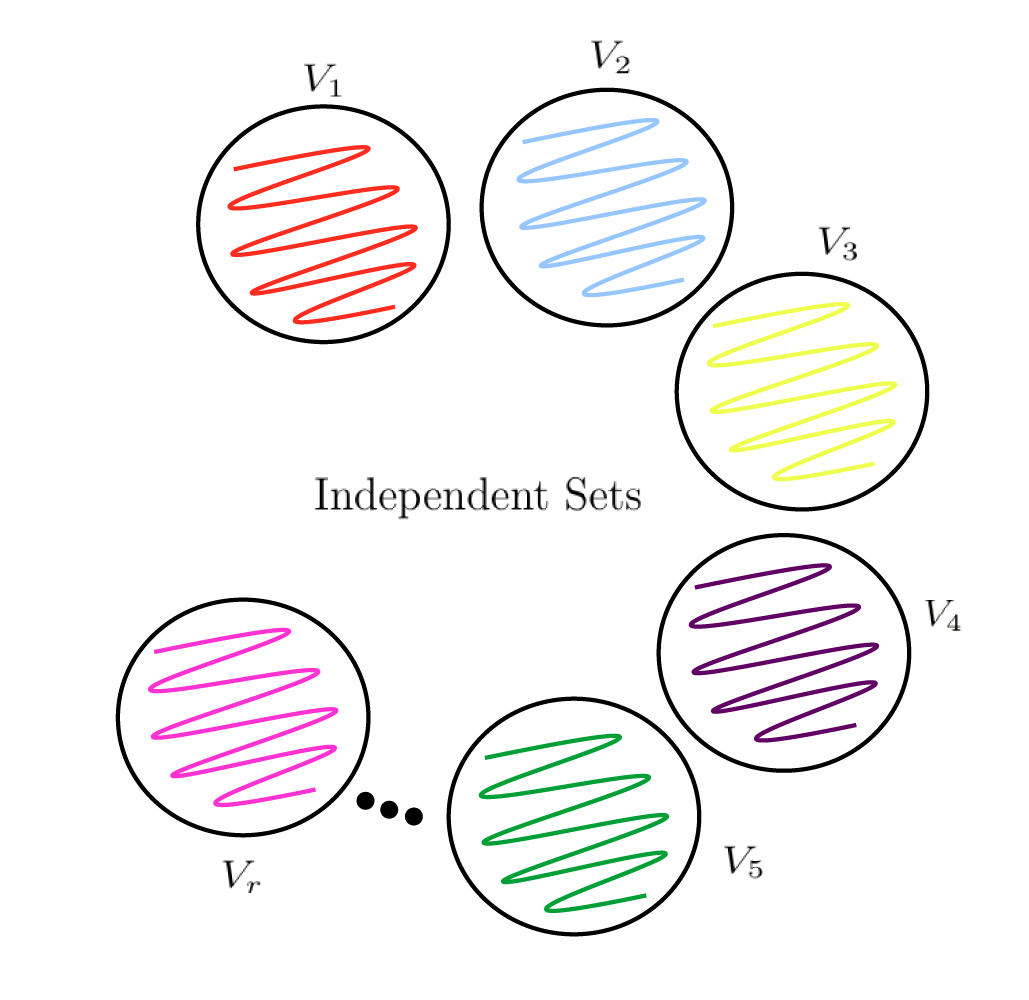
\includegraphics[scale=1]{Figuras/r-partion.jpg}
     \caption{r-coloring partition. }
     \label{fig:r-partition}
\end{figure}

By the pigeonhole principle we have $\alpha (G) \geq \frac{n}{r}$ and since $\mathbb{X}(G)=r$,

$$\mathbb{X}(G(n,p)) \geq \frac{n}{\alpha(G(n,p))},$$

and we want to show:

$$\mathbb{X}(G(n,p)) \geq \frac{n}{\alpha(G(n,p))} \geq k ,$$

Then,

$$\alpha(G(n,p)) < m \iff X_m=0 ,$$
with $X_m = \{|[A]|: S \in A$ if $S$ is a independent set with at least $m$ elements in $G(n,p)\}$,
and follows $m = \frac{n}{k}$. 

Being $S$ a independent set in $G(n,p)$ and $|S| \geq \frac{n}{k}$,

$$\mathbb{E}[X_m]=\sum_{\forall S\subset G(n,p)} \mathbb{P}(S) =(1-p)^{\binom{m}{2}} \binom{n}{m},$$
since we know that $\left(\frac{n}{m}\right)^m \leq \binom{n}{m} \leq \left(\frac{en}{m}\right)^m$ and $1-x \leq e^{-x}$ replacing in the equation above,

$$\mathbb{E}[X_m] \leq \left(\frac{en}{m}\right)^m  e^{(-pm^2)} = \left(\frac{en}{m} e^{(-pm)}\right)^m,$$

$$\mathbb{E}[X_m] \leq \left(\frac{en}{m} e^{(-pm)}\right)^m = \left(\frac{en}{m}\frac{1}{e^{(pm)}}\right)^m  << 1 \text{ if } e^{pm} >> n ,$$ 

as $m =\frac{n}{k}$,

$$ pn/k >> \log n \Rightarrow p >> \frac{k\log n}{n},$$
 
 By Markov's inequality,
 
 $$ \mathbb{P}(X_m \geq 1) \leq \mathbb{E}[X_m] ,$$
 
and if $p >> \frac{k \log n}{n},$
 
 $$ \mathbb{P}(X_m \geq 1) \leq \mathbb{E}[X_m] \leq \frac{1}{100}  \Rightarrow \mathbb{P}(\alpha (G(n,p)) < \frac{n}{k}) \geq \frac{99}{100} \Rightarrow $$

$$\mathbb{P}(\mathbb{X}(G(n,p)) > k) \geq \frac{99}{100}.$$


Since the proof for $\mathbb{X}(G) \geq k$ is finished we will prove $g(G)\geq k$,

$$ g(G(n,p)) \geq k \iff X_k \geq 1,$$


onde $X_k = |B|: $ todo $ C_k$ in $G(n,p) \in B$,

$$\mathbb{E}[X_k] = \sum_{\forall C_k \subset G(n,p)} \mathbb{P}(C_k)$$
\end{proof}

\chapter{Schedule}

\begin{table}[h]
\centering

\begin{tabular}{|r|lr|}
\hline
Task & Month&Year \\ 
\hline                               
Introduction, Methodology, Justification & August & 2018 \\
Chapter 1& September & 2018 \\
Chapter 2 &October & 2018 \\
Chapter 3&November & 2018 \\
 &December & 2018 \\
Chapter 4&January & 2019 \\
Chapter 5&February & 2019 \\
Conclusion&March & 2019 \\
Defense&April & 2019 \\
 &May & 2019   \\ 
\hline
\end{tabular}
\caption{Schedule.}
\label{tab:schedule}
\end{table}

\end{document}

%%% Local Variables:
%%% mode: latex
%%% eval: (auto-fill-mode t)
%%% eval: (LaTeX-math-mode t)
%%% eval: (flyspell-mode t)
%%% TeX-master: t
%%% En